\documentclass[a4paper,12pt]{article}
%%%%%%%%%%%%%%%%%%%%%%%%%%%%%%%%%%%%%%%%%%%%%%%%%%%%%%%%%%%%%%%%%%%%%%%%%%%%%%%%%%%%%%%%%%%%%%%%%%%%%%%%%%%%%%%%%%%%%%%%%%%%%%%%%%%%%%%%%%%%%%%%%%%%%%%%%%%%%%%%%%%%%%%%%%%%%%%%%%%%%%%%%%%%%%%%%%%%%%%%%%%%%%%%%%%%%%%%%%%%%%%%%%%%%%%%%%%%%%%%%%%%%%%%%%%%
\usepackage{eurosym}
\usepackage{vmargin}
\usepackage{amsmath}
\usepackage{graphics}
\usepackage{epsfig}
\usepackage{subfigure}
\usepackage{fancyhdr}
\usepackage{listings}
\usepackage{framed}
\usepackage{graphicx}
\usepackage{amsmath}
\usepackage{chngpage}
%\usepackage{bigints}

%\setcounter{MaxMatrixCols}{10}

\begin{document}
	\large
	%%-
\section*{Scatterplot for iris data set}
\begin{figure}[h!]
	\centering
	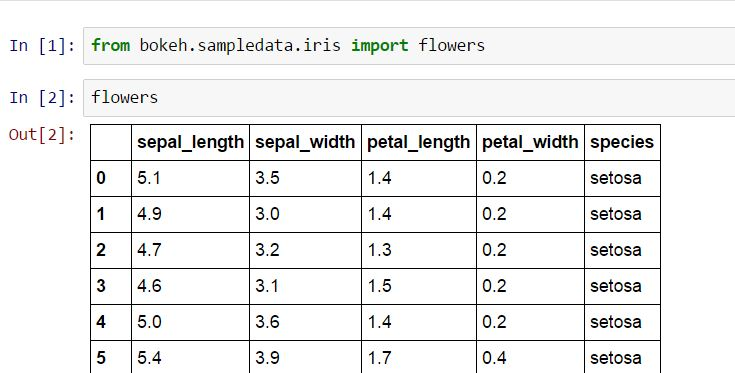
\includegraphics[width=0.8\linewidth]{images/iris-head}
\end{figure}
\begin{framed}
\begin{verbatim}
from bokeh.sampledata.iris import flowers
from bokeh.plotting import figure, show, output_file

colormap = {'setosa': 'red', 
            'versicolor': 'green', 
            'virginica': 'blue'}
flowers['color'] = 
     flowers['species'].map(lambda x: colormap[x])

output_file("iris.html", 
 title="iris.py example")

p = figure(title = "Iris Morphology")
p.xaxis.axis_label = 'Petal Length'
p.yaxis.axis_label = 'Petal Width'

p.circle(flowers["petal_length"],
        flowers["petal_width"],
        color=flowers["color"], 
        fill_alpha=0.2, size=10, )
show(p)
\end{verbatim}
\end{framed}
\newpage
\begin{figure}[h!]
\centering
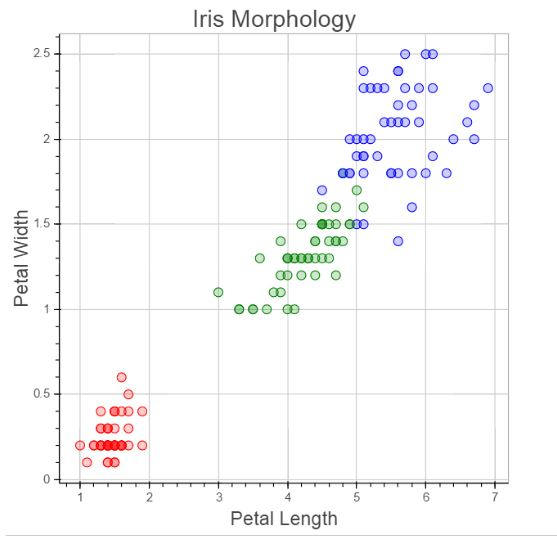
\includegraphics[width=0.6\linewidth]{images/02-iris-scatterplot1-petal}

\end{figure}
\subsection*{Exercises}
\begin{itemize}
\item Try this plot out for different combinations
of predictors variables.
\item Try out some different colour combinations for the \texttt{colormap}.
\item Try this out with a different data set : autompg. (\textit{See the graphic below.})  You can use \texttt{cyl} and \texttt{origin} as grouping variables. \begin{itemize}\item[$\ast$] The levels of cyl are 4,6 and 8. \item[$\ast$] The levels of origin are 1,2 and 3.
\end{itemize}
\end{itemize}
\begin{figure}[h!]
\centering
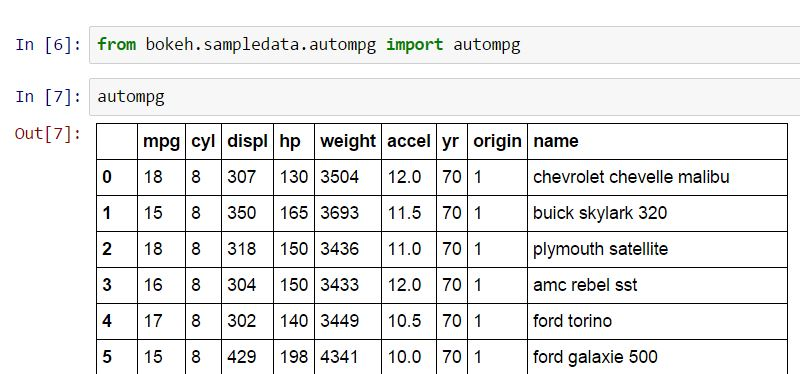
\includegraphics[width=0.9\linewidth]{images/autompg}
\end{figure}

\end{document}